\documentclass[11pt]{article}
\usepackage{graphicx}
\usepackage[margin=2.5cm]{geometry}
\usepackage{tikz}
\usepackage{indentfirst}
\usepackage{multirow, tabularx}
\usepackage{hyperref}
\usepackage{float}
\usepackage[portuguese]{babel}

\graphicspath{{./images/}}

\def\checkmark{\tikz\fill[scale=0.4](0,.35) -- (.25,0) -- (1,.7) -- (.25,.15) -- cycle;} 
\setlength{\parskip}{0.5em}

\hypersetup{
	colorlinks=false,
	linktoc=all,
	hidelinks,
}

\begin{document}
	\begin{titlepage}
	\begin{center}
		
\includegraphics[width=0.6\textwidth]{logo-isec}
		
		\vspace*{\fill}
		
		\Huge
		\textbf{Interação Pessoa-Máquina}
		
		\huge
		Avaliação da Interface de dispositivos
		
		\vspace{0.5cm}
		\LARGE
		2020 - 2021
		
		\vspace{1.5cm}
		
		\textbf{TheForgotten\\merlin-twist}
		
		\begin{figure}[h]
			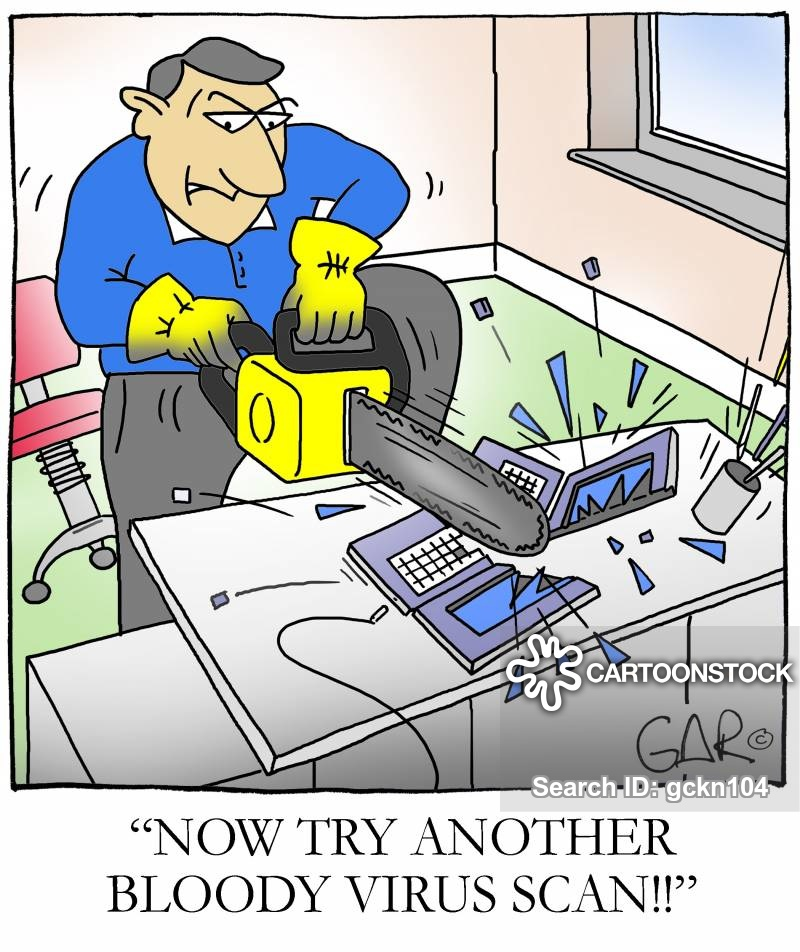
\includegraphics[width=0.5\textwidth]{boomer}
			\centering
			\caption{Homem irritado com o computador}
			\label{fig:angry-man}
		\end{figure}
		
		\vfill
		\vspace*{\fill}
		
		\normalsize
		Licenciatura de Engenharia Informática \\
		5 de março de 2021		
	\end{center}
\end{titlepage}
	
	\tableofcontents
	\pagebreak
	
	\large
	\section{Introdução}
	\normalsize
	
	Este trabalho consiste na especificação e implementação da interface gráfica e respetiva interação de uma aplicação. A aplicação que iremos desenvolver pretende fornecer uma experiência de leitura de ebooks melhor usando a tecnologia de realidade virtual. 
	
	Assim, ao invés de simplesmente olharmos para um ecrã com texto, existiria todo um espaço virtual por onde poderíamos navegar e ler livros, passando a interação de um simples scroll para algo bem mais rico.
	

	\large
	\section{Análise de Utilizadores}
	\normalsize
	
	Usando o método das \textbf{Personas} criado por Alan Cooper, podemos traçar 4 grandes grupos de utilizadores da nossa aplicação. Estas vão ser baseadas em dados recolhidos de pessoas à nossa volta que experimentaram a nossa aplicação através de questionários e observação.
	
	\begin{tabularx}{\textwidth}{|X|}
		\hline
		\textbf{João Silva} \\
		\textbf{O universitário relaxado} \\
		\hline
		\hspace{5mm} - Estuda na universidade, faz 2 cadeiras por semestre \\
		\hspace{5mm} - Vive relaxadamente e sem pressas \\
		\hspace{5mm} - Defende que o importante é a jornada e não o destino \\
		\hspace{5mm} - Não tem responsabilidades \\
		\hspace{5mm} - Fica enervado quando as coisas não funcionam como deviam \\
		\hspace{5mm} - Dá prioridade a uma boa experiência de utilização e não a algo eficiente \\
		\hline
	\end{tabularx}

	\begin{tabularx}{\textwidth}{|X|}
		\hline
		\textbf{Ambrósio Mota} \\
		\textbf{O adulto apressado} \\
		\hline
		\hspace{5mm} - Trabalha 5 dias por semana, 10h por dia \\
		\hspace{5mm} - Gosta de coisas rápidas e eficientes \\
		\hspace{5mm} - Não tem olhar para apreciar um bom design \\
		\hspace{5mm} - Anda sempre muito atarefado, tem pouco tempo livre \\
		\hspace{5mm} - Gosta de ler um pouco antes de dormir \\
		\hspace{5mm} - Não se sente totalmente confortável com as novas tecnologias \\
		\hline
	\end{tabularx}

	\begin{tabularx}{\textwidth}{|X|}
		\hline
		\textbf{Susana Pinheiro} \\
		\textbf{A super mãe} \\
		\hline
		\hspace{5mm} - Mantém a casa limpa e arrumada \\
		\hspace{5mm} - Parece que controla o tempo pois arranja sempre maneira de fazer tudo \\
		\hspace{5mm} - Tem 3 filhos para educar \\
		\hspace{5mm} - Aprecia arte e quando tem tempo gosta de visitar exposições \\
		\hspace{5mm} - Não perde um episódio das novelas brasileiras \\
		\hspace{5mm} - Tem cartão de desconto para todos os supermercados imagináveis \\
		\hline
	\end{tabularx}

	\begin{tabularx}{\textwidth}{|X|}
		\hline
		\textbf{Maurício Pires} \\
		\textbf{O futuro da nação} \\
		\hline
		\hspace{5mm} - Joga "à bola" todos os dias depois da escola \\
		\hspace{5mm} - Está no 5° ano e gosta muito de ciências \\
		\hspace{5mm} - Joga fortnite a noite inteira até a mãe lhe desligar a internet \\
		\hspace{5mm} - Teve um contacto muito reduzido com livros \\
		\hspace{5mm} - Qualquer aplicação que não seja interativa e "mexida" não capta a atenção dele por mais do que 5 segundos \\
		\hspace{5mm} - Não tem preocupações \\
		\hline
	\end{tabularx}	

	O João Silva e o Maurício Pires representam o nosso grande foco, mas é também importante dar atenção à Susana e ao Ambrósio pois estes representam um grande número de utilizadores.

	
	\large
	\section{Análise de Tarefas}
	\normalsize
	
	Usando a abordagem top-down, podemos deliniar tarefas partindo do objetivo principal.
	
	\begin{itemize}
		\item \textbf{Objetivo principal:} ler um ebook
		\item \textbf{Tarefas:}
		\begin{itemize}
			\item escolher o ebook duma lista
			\item escolher o ebook duma prateleira
			\item importar ebooks
			\item comprar ebooks
		\end{itemize}
	\end{itemize}
	
	Assim, teremos as seguintes tarefas:
	
	\begin{itemize}
		\item \textbf{Objetivo:} escolher o ebook da lista
		\item Pré-condições: encontrar-se no espaço de aplicação para leitura
		\item Sub-tarefas:
		\begin{itemize}
			\item Abrir a lista de ebooks a que tem acesso
		\end{itemize}
	\end{itemize}

	\begin{figure}[H]
		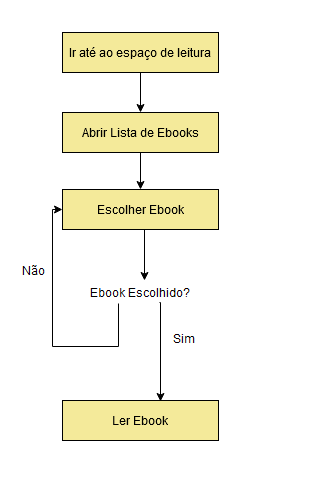
\includegraphics[width=0.25\textwidth,height=0.88\textheight,keepaspectratio]{tarefa-listar-ebook}
		\centering
		\caption{Análise Sequencial - Escolher o ebook da lista}
		\label{fig:as-escolherLista}
	\end{figure}

	\begin{itemize}
		\item \textbf{Objetivo:} escolher o ebook duma prateleira
		\item Pré-condições: encontrar-se no espaço de aplicação para leitura
		\item Sub-tarefas:
		\begin{itemize}
			\item Dirigir-se à prateleira
			\item "Agarrar" no livro desejado
			\item Voltar para o local de leitura
		\end{itemize}
	\end{itemize}

	\begin{figure}[H]
		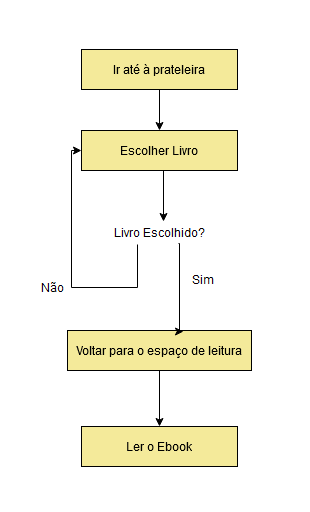
\includegraphics[width=0.25\textwidth,height=0.88\textheight,keepaspectratio]{tarefa-livro-prateleira}
		\centering
		\caption{Análise Sequencial - Escolher o ebook duma prateleira}
		\label{fig:as-escolherPrateleira}
	\end{figure}

	\begin{itemize}
		\item \textbf{Objetivo:} importar ebook
		\item Pré-condições: estar no menu de importação de ebooks, possuir o ebook no dispositivo
		\item Sub-tarefas:
		\begin{itemize}
			\item Selecionar o ficheiro do ebook
		\end{itemize}
	\end{itemize}

	\begin{figure}[H]
		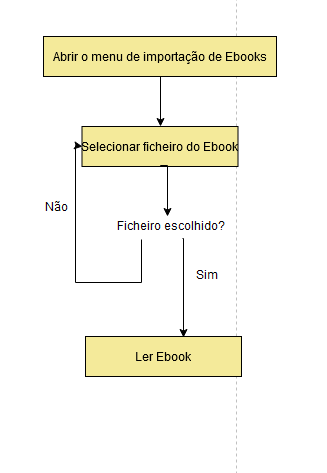
\includegraphics[width=0.25\textwidth,height=0.88\textheight,keepaspectratio]{tarefa-importar-ebook}
		\centering
		\caption{Análise Sequencial - Importar ebook}
		\label{fig:as-importarEbooks}
	\end{figure}

	\begin{itemize}
		\item \textbf{Objetivo:} comprar ebook
		\item Pré-condições: estar no menu de compra de ebooks
		\item Sub-tarefas:
		\begin{itemize}
			\item Selecionar o ebook que deseja comprar
			\item Pagar o livro
		\end{itemize}
	\end{itemize}

	\begin{figure}[H]
		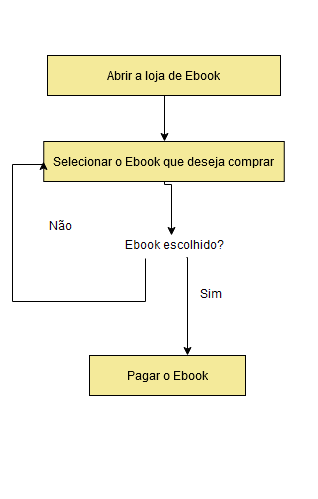
\includegraphics[width=0.25\textwidth,height=0.88\textheight,keepaspectratio]{tarefa-comprar-ebook}
		\centering
		\caption{Análise Sequencial - Comprar ebook}
		\label{fig:as-comprarEbook}
	\end{figure}
	
	\large
	\section{Metáforas}
	\normalsize
	
	Sendo uma aplicação em realidade virtual que pretende emular a experiência de leitura que se teria numa biblioteca e na "vida real", esta é repleta de metáforas.
	
	O utilizador pode pegar em livros da mesma forma que o faria num contexto real, podendo folhear e ouvir as páginas a serem manipuladas tal como aconteceria fora da aplicação.
	
	Para representar e organizar os ebooks são usados livros e estantes, elementos que remetem para uma biblioteca.
	
	Na loja, associado à compra, temos um carrinho de compras a servir de botão, tal como temos os carrinhos nos supermercados.
	
	Para além de pegar nos livros acabará também por ler da mesma maneira que faria fora do contexto da aplicação.
	
	Poderá caminhar no ambiente tal como caminharia num ambiente real.
	
	
	\large
	\section{Protótipo}
	\normalsize
	
	Usando o Balsamiq, fizemos o seguinte protótipo de baixa fidelidade. Contém as principais funcionalidades da aplicação e o aspeto que, de um modo geral, estas devem ter.
	
	\begin{figure}[H]
		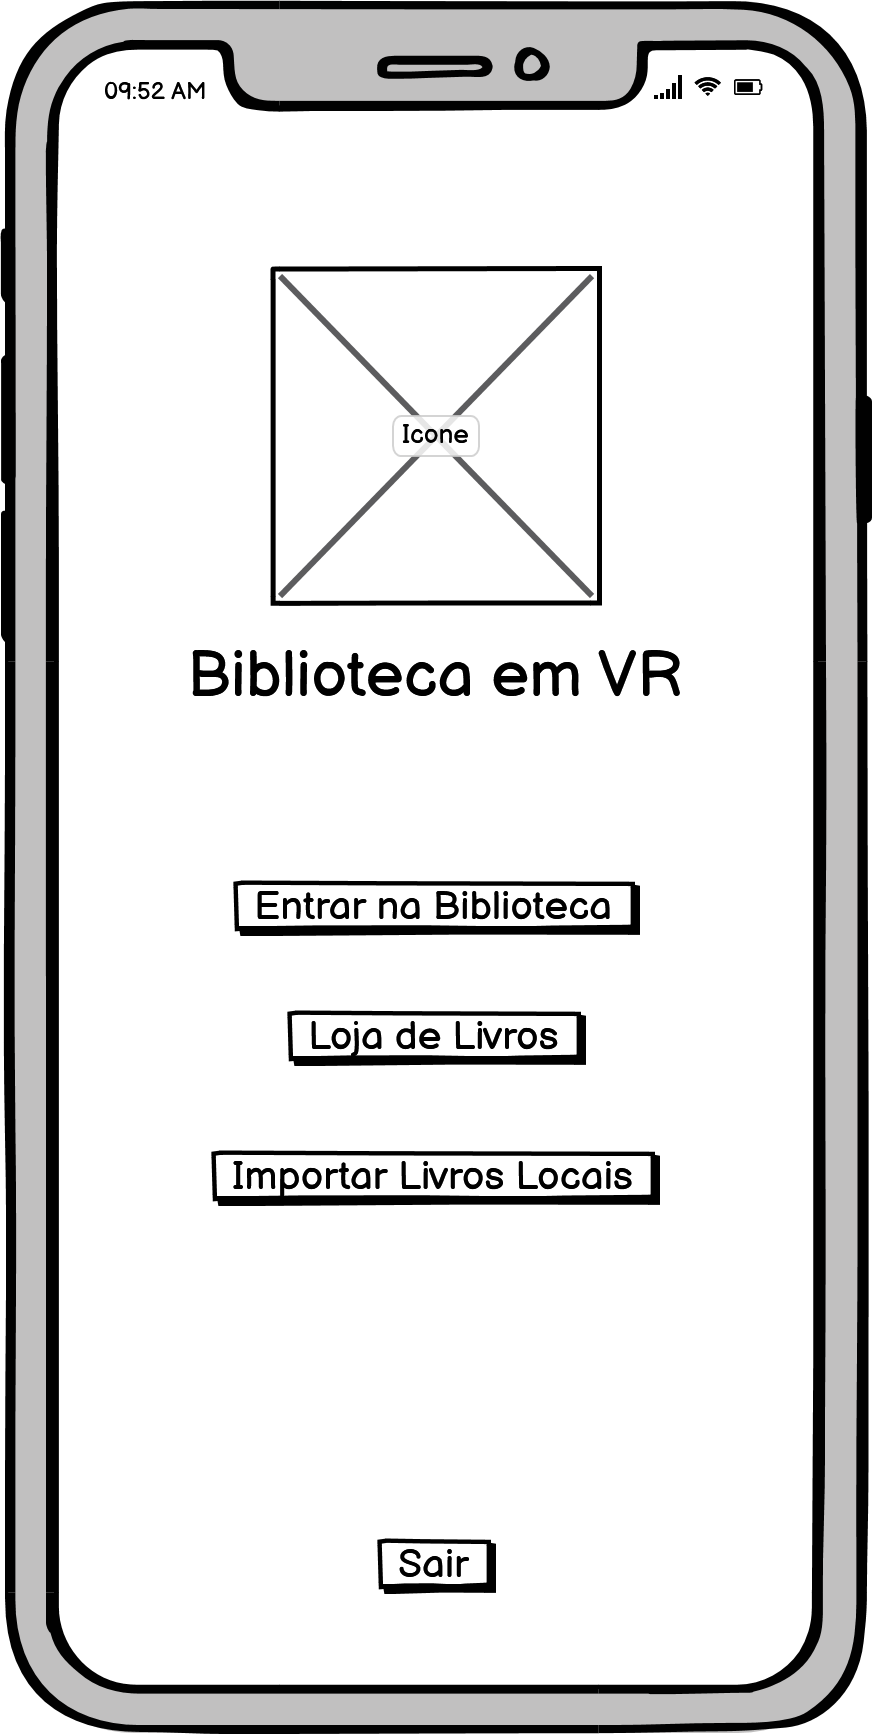
\includegraphics[width=0.25\textwidth,height=0.88\textheight,keepaspectratio]{main-menu}
		\centering
		\caption{Menu Principal}
		\label{fig:menu}
	\end{figure}

	Este é o menu principal. Aqui o utilizador escolhe o que pretende fazer. É simples e intuitívo de maneira a que qualquer um possa usar.
	
	\begin{figure}[H]
		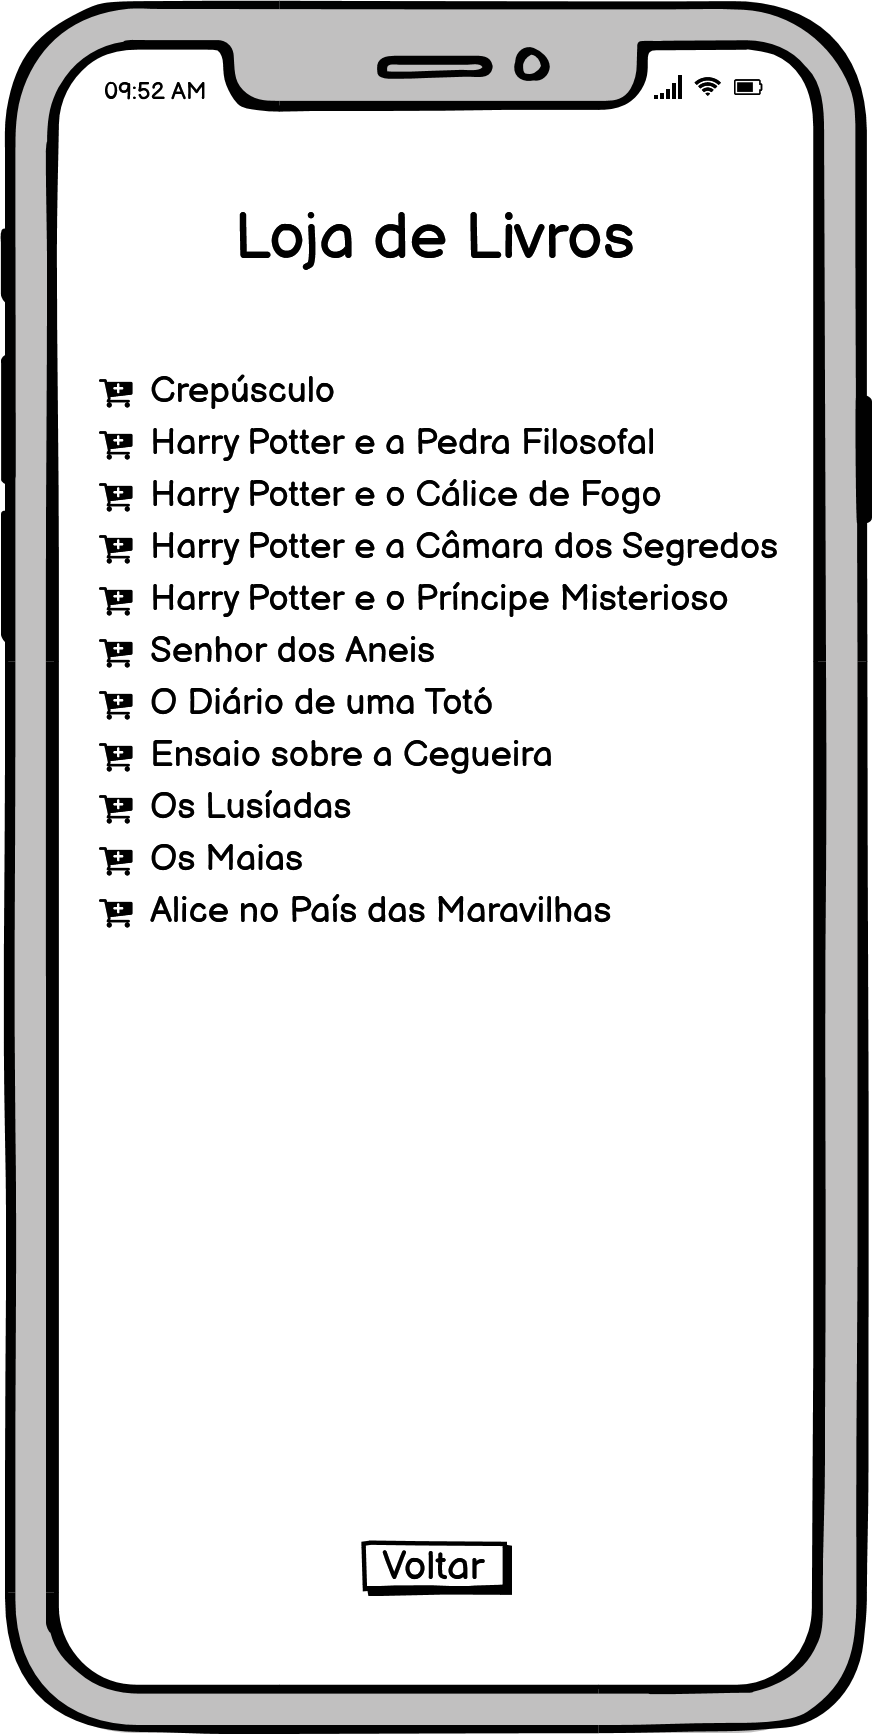
\includegraphics[width=0.25\textwidth,height=0.88\textheight,keepaspectratio]{loja-livros}
		\centering
		\caption{Loja de Livros}
		\label{fig:loja}
	\end{figure}

	Aqui o utilizador pode adquirir mais livros. Para tal, apenas precisa de clicar no ícone do lado esquerdo do título.
	
	\begin{figure}[H]
		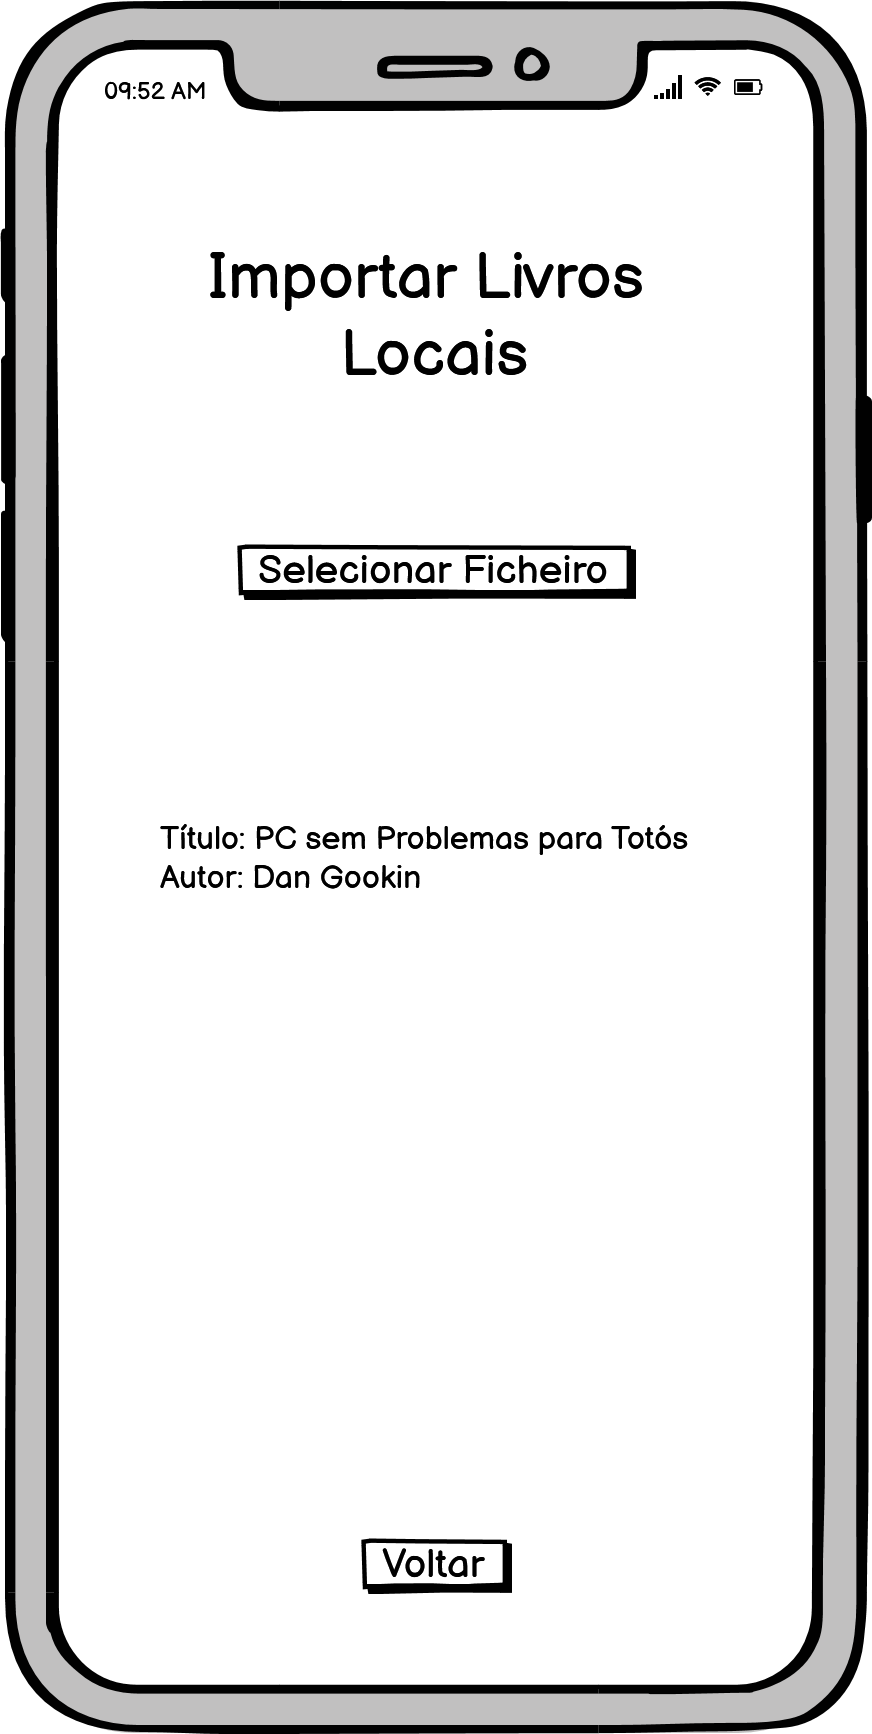
\includegraphics[width=0.25\textwidth,height=0.88\textheight,keepaspectratio]{importar-livros}
		\centering
		\caption{Importar Livros Locais}
		\label{fig:importar}
	\end{figure}
	
	De modo a não descartar a possibilidade de o utilizador ter adquirido o livro noutra plataforma e ter acesso a ele localmente, a aplicação oferece também uma maneira de importar esses ebooks. Isto é também útil para poder ter acesso a livros que são gratuitos e distribuídos neste formato.
	
	A informação como título e autores é retirada do próprio ficheiro, dando possibilidade ao utilizador de alterar caso esta se encontre errada.

	\begin{figure}[H]
		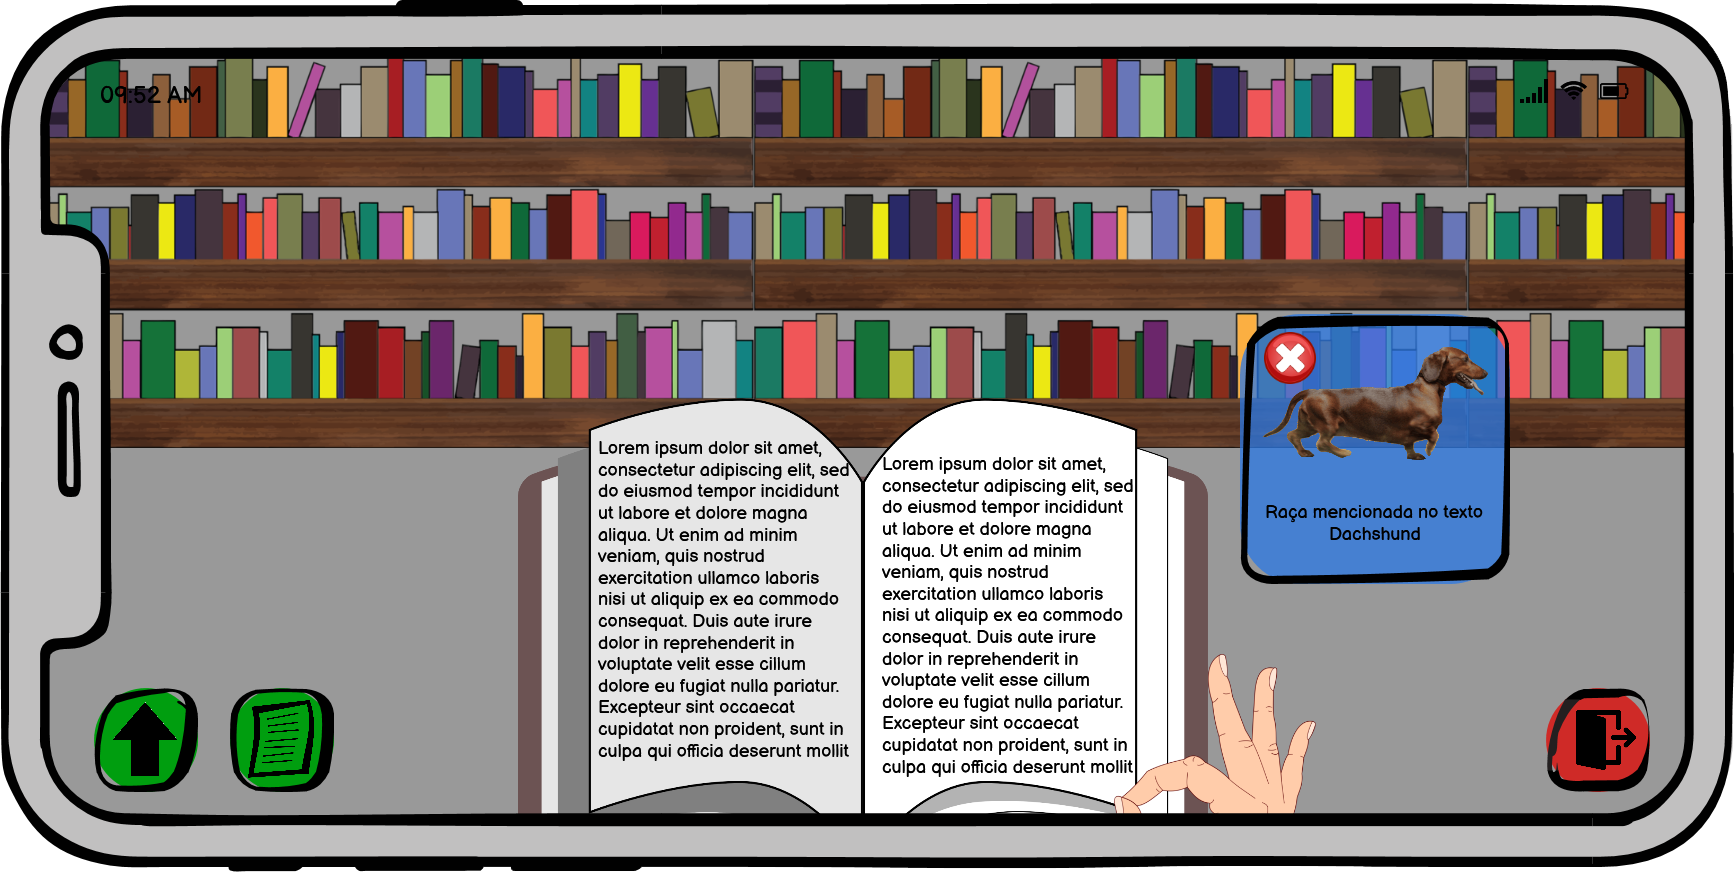
\includegraphics[width=0.95\textwidth,height=0.25\textheight,keepaspectratio]{biblio-ler}
		\centering
		\caption{Exemplo de Leitura}
		\label{fig:leitura}
	\end{figure}

	Este é o aspeto geral da aplicação quando o utilizador está a ler. A interação com os botões é feita com o olhar, ou seja, se ficarmos a olhar para os botões durante 3 segundos estes vão ser acionados. Isto é simples de fazer com a tecnologia de realidade virtual ncessária para a aplicação e assim podemos tornar a utilização mais fácil e intuitiva.
	
	O botão mais à esquerda indica ao utilizador para se levantar, daí a seta a apontar para cima. O botão à direita desse é para abrir a lista de livros que o utilizador pode ler. Por fim, o botão à direita é para voltar ao menu inicial.
	
	Deste modo, para mudar de página, se o utilizador não possuir nenhum equipamento especial para simular esta interação, pode apenas olhar para o canto da páginas que esta irá virar.
	
	\begin{figure}[H]
		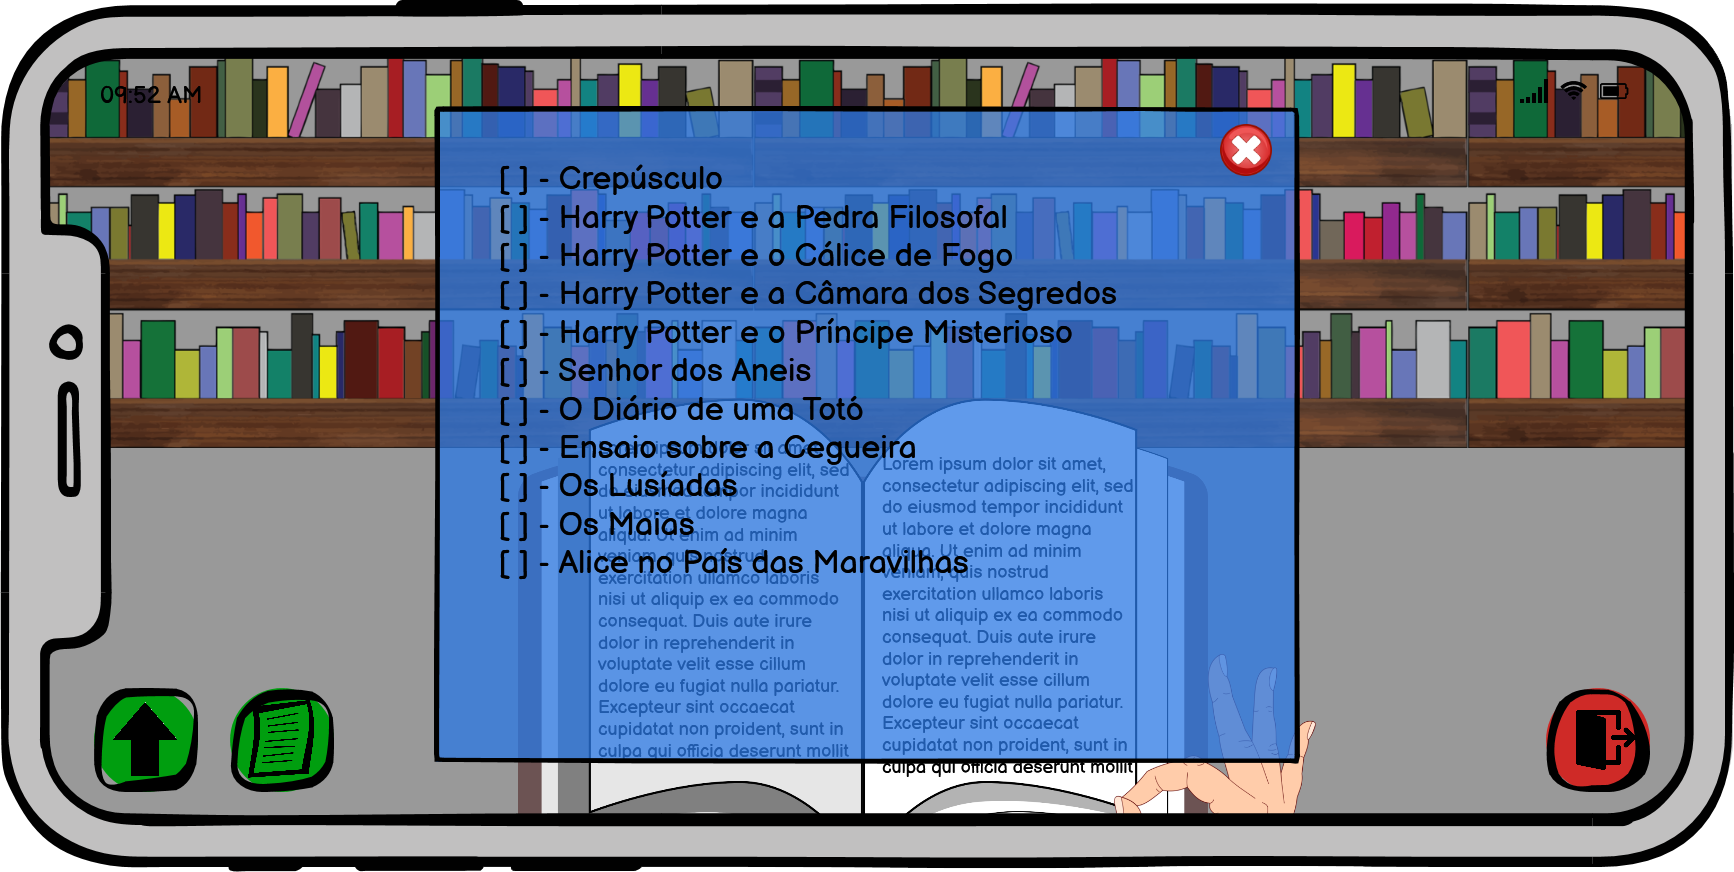
\includegraphics[width=0.95\textwidth,height=0.25\textheight,keepaspectratio]{biblio-escolher-lista}
		\centering
		\caption{Exemplo de Lista}
		\label{fig:lista}
	\end{figure}
	
	Aqui podemos ver o aspeto da lista de livros. Esta opção existe para satisfazer o Ambrósio que tá sempre com muita pressa.
	
	Para selecionar um livro basta olhar para a caixa à esquerda do título.
	
	\begin{figure}[H]
		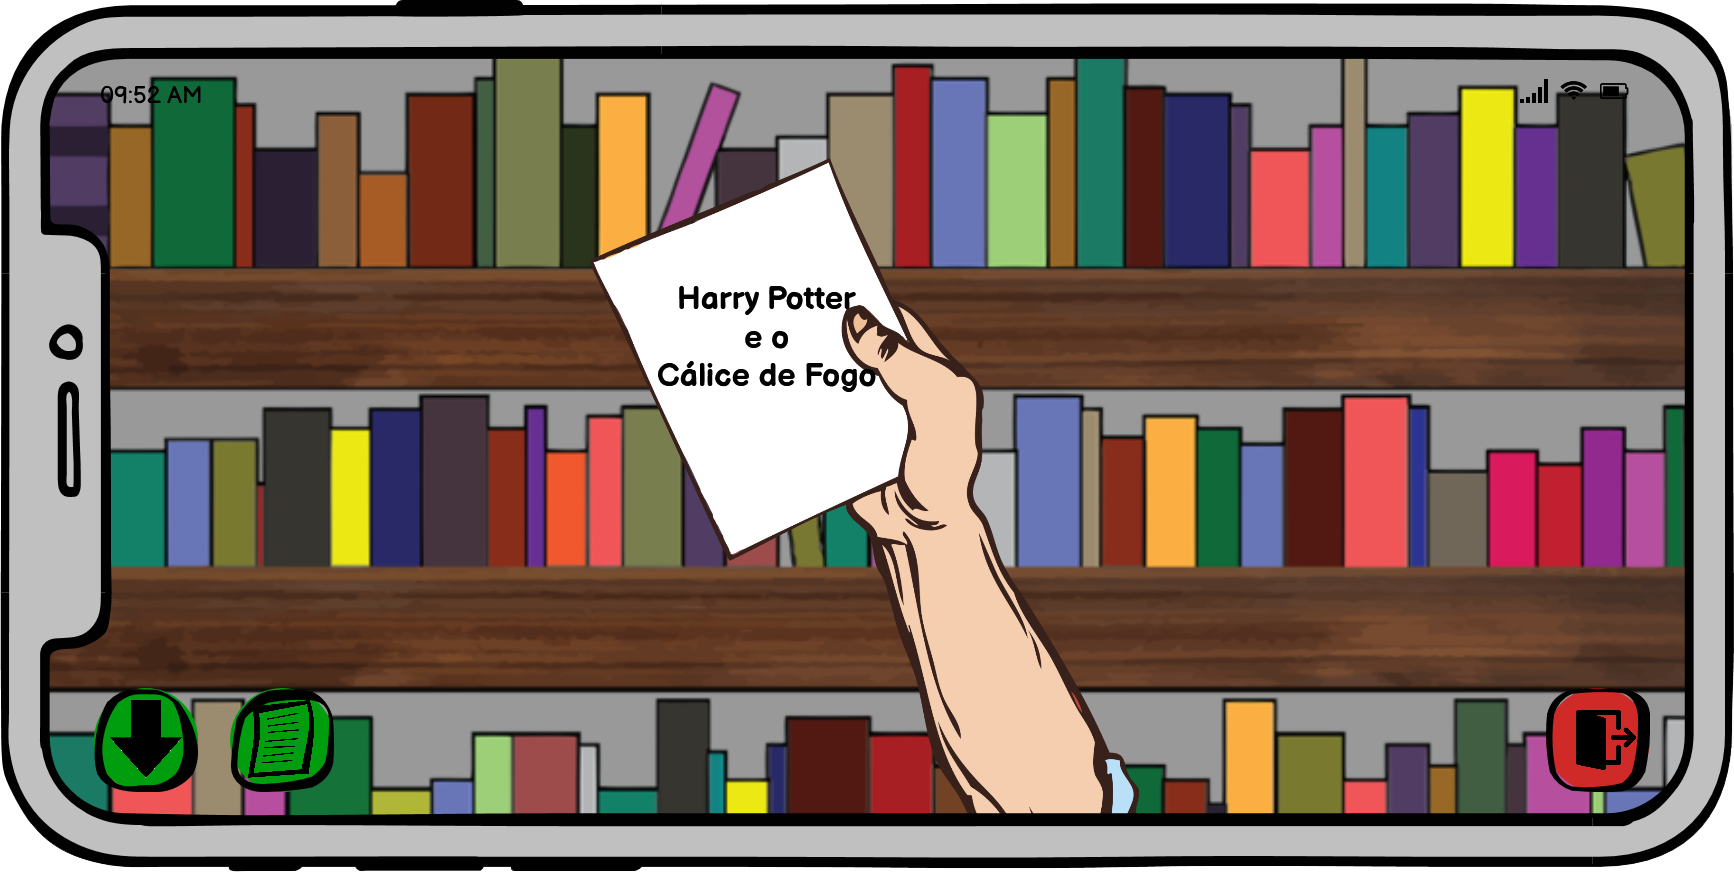
\includegraphics[width=0.95\textwidth,height=0.25\textheight,keepaspectratio]{biblio-escolher-prateleira}
		\centering
		\caption{Exemplo de Prateleira}
		\label{fig:prateleira}
	\end{figure}

	Aqui é possível perceber como funciona a funcionalidade de pegar um livro numa prateleira. Esta tarefa faz parte do foco principal da aplicação que é fornecer uma experiência parecida à de estar numa biblioteca física.
	
	Como podemos ver, o botão de levantar tem agora a seta invertida, porque, como o utilizador se encontra levantado, agora o botão serve para ele se puder sentar.
	
	Os livros pode ser escolhido da prateleira da mesma maneira que interagímos com o resto da aplicação, ou seja, olhar fixamente durante 3 segundos para o que queremos.
	
	Desta maneira, podemos fornecer uma boa experiência de navegação de um espaço como biblioteca e de leitura no mesmo num mundo virtualizado. O utilizador poderá levantar-se e pegar o livro que quer ou, se for apressado, escolher duma lista. Para além disso, da maneira que os controlos estão desenhados, qualquer um consegue facilmente se localizar na aplicação. 
	
	\large
	\section{O Design da Aplicação}
	\normalsize
	
	A aplicação foi pensada para fornecer uma ótima experiência ao utilizador, não só do ponto de vista de utilidade como do ponto de vista de usabilidade, de maneira a tentar agradar não só o João Silva como o Ambrósio Mota.
	
	Os menus são simples e intuítivos e sem caminho inflexíveis, dando uso a uma linguagem que qualquer utilizador conseguirá entender. Optamos por um design minimalista pois não só é mais esteticamente apelativo como também facilita o uso da aplicação, eliminando assim a necessidade de algum tipo de tutorial ou documentação.
	
	Durante a utilização do ambiente de leitura, o menu de acesso rápido possuí apenas os botões necessários e importantes, com ícones que ilustram bem o que significam. Para além disso, usam também cores diferentes para distinguir as suas funcionalidades, ficando o vermelho reservado para a opção de saída e o verde para as funcionalidades. No caso do utilizador ser daltónico este terá a opção de ativar um modo onde as cores mudariam para algo mais adequado para o seu tipo de daltonismo.
	
	
	\large
	\section{Acessibilidade}
	\normalsize
	
	A nossa aplicação abrange um grande grupo de pessoas com necessidades.
	
	Considerando pessoas com dificuldades motoras, o facto de oferecer um espaço virtual onde nos podemos movimentar sem na verdade nos mexermos tornará este projeto muito interessante para pessoas que não se conseguem movimentar sozinhas e se queiram sentir mais livres. Tendo em conta também paraplégicos, com os controlos simples que a aplicação oferece recorrendo ao uso do olhar para movimentar e realizar todas as ações, seria também uma nova maneira de estes se puderem sentir mais independentes.
	
	Pensando também em pessoas com défice de atenção, por exemplo, o facto de haver animações ou até um ambiente todo em volta da experiência de leitura acabará por também facilitar manter a atenção à leitura.
	
	Por fim, facilmente conseguimos implementar um modo daltónico para as pessoas que sofrem de daltonismo se puderem sentir mais confortáveis no ambiente que a nossa aplicação fornece.
	
	
	\large
	\section{Protótipo de Alta Fidelidade / Implementação Inicial}
	\normalsize
	
	Em anexo vai a aplicação preparada para usar com Google Cardboard. O ficheiro \textit{.apk} deve ser instalado num smartphone com android 4.4 ou superior.
	
	Esta implementação foi feita em Unity, software que não aprendemos a usar durante o curso.
	
	Apesar de não ser complicado uma pequena implementação para usar com Cardboard em Unity, tentamos programar a movimentação e o menu mas, devido à nossa falta de conhecimento e à vontade com o software não fomos capazes de implementar.
	
	Ainda assim, o utilizador vai estar num ambiente tipo biblioteca (muito cru e pouco detalhado), sentado numa cadeira de madeira e com um livro ao colo. Desta maneira já pode ter uma boa noção de como é a experiência da leitura em VR (se possuir o Google Cardboard, claro).
	
	\begin{figure}[H]
		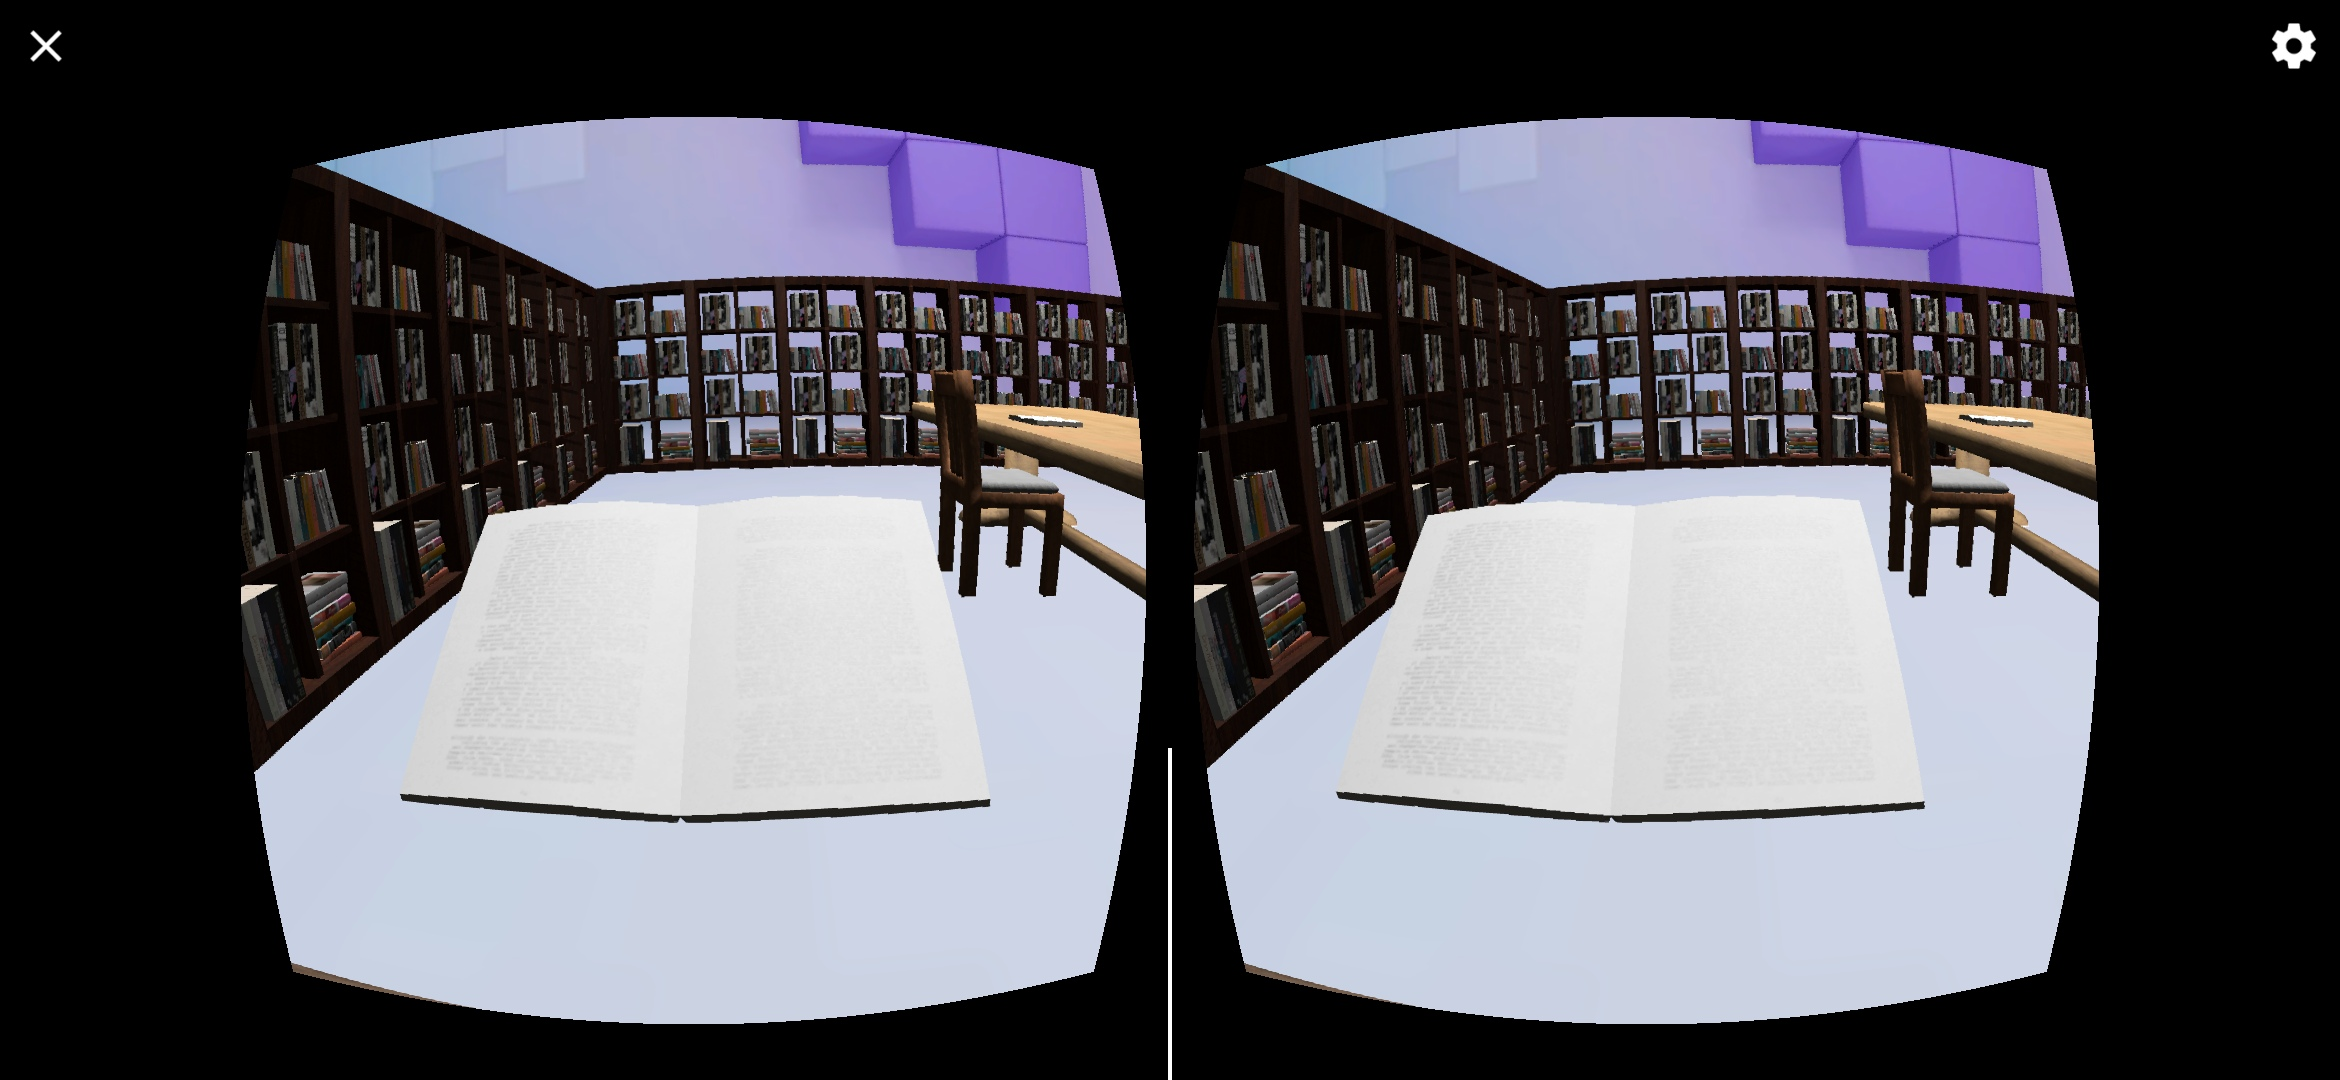
\includegraphics[width=0.95\textwidth,height=0.88\textheight,keepaspectratio]{print-app}
		\centering
		\caption{Captura da Aplicação}
		\label{fig:print-app}
	\end{figure}
	
	
	\large
	\section{Ligação com Óculos de Realidade Virtual}
	\normalsize
	
	Apesar da nossa implementação inicial ter sido feita para Google Cardboard como mencionado, facilmente se torna a aplicação compatível com qualquer tipo de óculos de realidade virtual pois o Unity facilita este processo, sendo para o efeito necessário modificar muito pouco.
	
	Com o uso de uns óculos que tivessem controlos poderiam ser dadas mais funcionalidades à aplicação como, por exemplo, interagir de alguma maneira diferente com as informações extras que aparecem sobre o que estamos a ler. Se aparecesse, por exemplo, um cão, poderia ser dada a possibilidade de acaraciar o mesmo.
	
	O Unity facilita imenso o processo de fazer a aplicação para todo o tipo de plataformas e de adicionar suporte para um variado número de tecnologias.

	
	\large
	\section{Conclusão}
	
	\normalsize
	Temos confiança de que temos uma boa proposta.
	
	Não só é inovadora pois não conseguimos encontrar nada que fizesse o que pretendemos fazer, como também ajudará imensas pessoas com necessidades especiais.
	
	Para além disso é também uma excelente maneira de voltar a despertar o interesse pela leitura nas pessoas que já tinham perdido o gosto. No entanto, não podemos esquecer também a geração que cresceu num mundo totalmente digital, que nunca tendo tido grande amor ou necessidade de ler livros, poderiam ficar atraídos pela nossa elegante solução e assim entrar no brilhante mundo dos livros.
	
	
	\pagebreak
	
	\large
	\section{Anexos}

	\normalsize
	\listoffigures
\end{document}